\chapter[Prefácio, \textit{por Celso Lafer}]{Prefácio \subtitulo{O próximo e o distante}}
\hedramarkboth{Prefácio}{}

\begin{flushright}
\textsc{celso lafer}
\end{flushright}

\section*{A Jerusalém da Lituânia}

\noindent{}Escrever sobre uma cidade procurando desvendar seu significado é uma
tarefa difícil e desafiante. Exige múltiplos conhecimentos, antenas de
compreensão e sensibilidade, conjugados com os talentos de um escritor.
É o que faz de qualificadas obras sobre o tema um gênero literário
próprio. É o caso, por exemplo, nas letras brasileiras, de \textit{Amor a
Roma}, de Afonso Arinos, \textit{Paris, a capital do século \textsc{xix}},
de Walter Benjamin, e \textit{Jerusalém: a biografia}, de Simon Sebag
Montefiore.

O livro de Laimonas Briedis, publicado em inglês em 2016, cuja edição
brasileira tenho a satisfação de prefaciar, insere"-se no patamar desse
gênero literário. Em sua elaboração, o autor enfrentou com sucesso
muitos desafios.

O primeiro deles foi a capacidade de transmitir o significado de uma
cidade que viveu no limiar da Europa, um espaço geográfico e cultural de
múltiplas dimensões e que, à primeira vista, não possui a \textit{vis
atractiva} de uma ``cidade eterna'' como Roma, ou de uma ``cidade luz''
como Paris. Para o leitor brasileiro, é uma cidade distante do Báltico,
próxima do ``congelado inverno'' do \textit{Sarmático Oceano} para valer"-me da
narrativa de Camões sobre a geografia da Europa em \textit{Os Lusíadas}\footnote{Canto \textsc{iii}, estrofe 9.}. É um limiar no âmbito interno da Europa profunda. Contrasta
com o ``Reino Lusitano/\,onde a terra se acaba e o mar começa'', que é
para o poeta ``quase cume da cabeça/\,da Europa toda''\footnote{Canto \textsc{iii}, estrofe 20}. 
É do ``olhar mundo'' do cume da cabeça da Europa da
épica camoniana que provém a matriz lusitana, originária do país que é
hoje o Brasil. Ter sabido tornar próximo o distante para um leitor
brasileiro, é o primeiro mérito do livro de Laimonas Briedis que cabe
destacar.

O deslinde desse distante, para torná"-lo inteligível, é, por sua vez,
extremamente complexo, uma complexidade constitutiva do cerne das
dificuldades que Laimonas Briedis enfrentou na concepção e na elaboração
de seu livro.

\textit{\textit{Vilnius}} é hoje a capital da Lituânia. O fim da União Soviética e as
transformações econômicas e políticas, que dela derivaram, assinalaram o
término das relevâncias geopolíticas da Europa Oriental como um
componente da Guerra Fria. Nessa nova moldura, a Lituânia tornou"-se um
país independente, dotado de autonomia na condução de sua política e na
gestão de seus assuntos internos. É uma cidade demograficamente lituana
e de fala lituana.

Esta é, no entanto, uma nova realidade no percurso histórico de uma
cidade muito impregnada, em seus componentes medievais, pelo barroco,
que viveu no limiar da Europa e no contexto de suas mudanças
cartográficas, e cujos habitantes de diversas origens, por isso mesmo,
percorreram suas casas e ruas, falando, sucessiva ou concomitantemente,
várias línguas. Articularam, assim, em diversos idiomas, suas vivências
e memórias.

A cidade foi por isso mesmo um \textit{locus} paradigmático da
\textit{heteroglossia}, termo cunhado e teoricamente elaborado pelo grande
crítico russo Mikhail Bakhtin. Bakhtin viveu sua juventude em Vilna, de
1904 a 1912, quando seu pai integrava a administração russa da cidade.
Provavelmente, inspirou"-se em sua vivência ali, como sugere Laimonas
Briedis, para a elaboração teórica a respeito das correlações temporais
e espaciais de vários âmbitos linguísticos.

\textit{\textit{Vilnius}} foi \textit{Vilna}, denominação em eslavo, que assinala a longa
eslava presença no tempo na cidade da Rússia czarista e soviética.
Também foi \textit{Wilno} para os poloneses, o que realça o histórico
relacionamento da Lituânia e da Polônia, que está na origem política dos
dois países. Também foi \textit{Wilna} para os alemães, que tiveram relevantes
passagens nas incursões da Alemanha no Leste Europeu pela cidade. Para
os judeus \textit{ashkenazim}, foi, em iídiche, \textit{Vilnè}, a irradiadora
Jerusalém da Lituânia no mundo judaico, identificadora das
características culturais e religiosas de seus \textit{litvaks}, que,
dizimados pelo Holocausto, desapareceram da cidade.

Esta problematicidade se revela no título do livro de Laimonas Briedis,
no original inglês, \textit{\textit{Vilnius}, City of Strangers}, e na tradução
para o português, \textit{Vilna, cidade dos outros}, que se deve aos
cuidados de Fernando Klabin e, ao optar pela forma \textit{Vilna}, ecoa o nome
da cidade no final do século \textsc{xix}, quando a família Klabin imigrou da
Lituânia e encontrou seu destino no Brasil.

Czeslaw Miłosz, grande poeta da língua polonesa, prêmio Nobel de
Literatura que nasceu na Lituânia e estudou em Vilna, intitula, não por
acaso, um de seus poemas ``City without name'', que começa indagando
``Who will honor the city without a name/\,if so many are
dead\ldots{}''.\footnote{Czeslaw Miłosz. \textit{Selected and Last Poems ---
  1931--2004}. Seleta de Robert Hass e Anthony Miłosz. Nova York: Harper
  Collins; Ecco Paperback Edition, 2011, p. 261. O verso, que pode ser traduzido como ``Cidade sem nome'', 
  diz: ``Quem honrará a cidade sem nome/\,se tantos estão mortos\dots{}.''}

\begin{figure}[!ht]
    \centering
    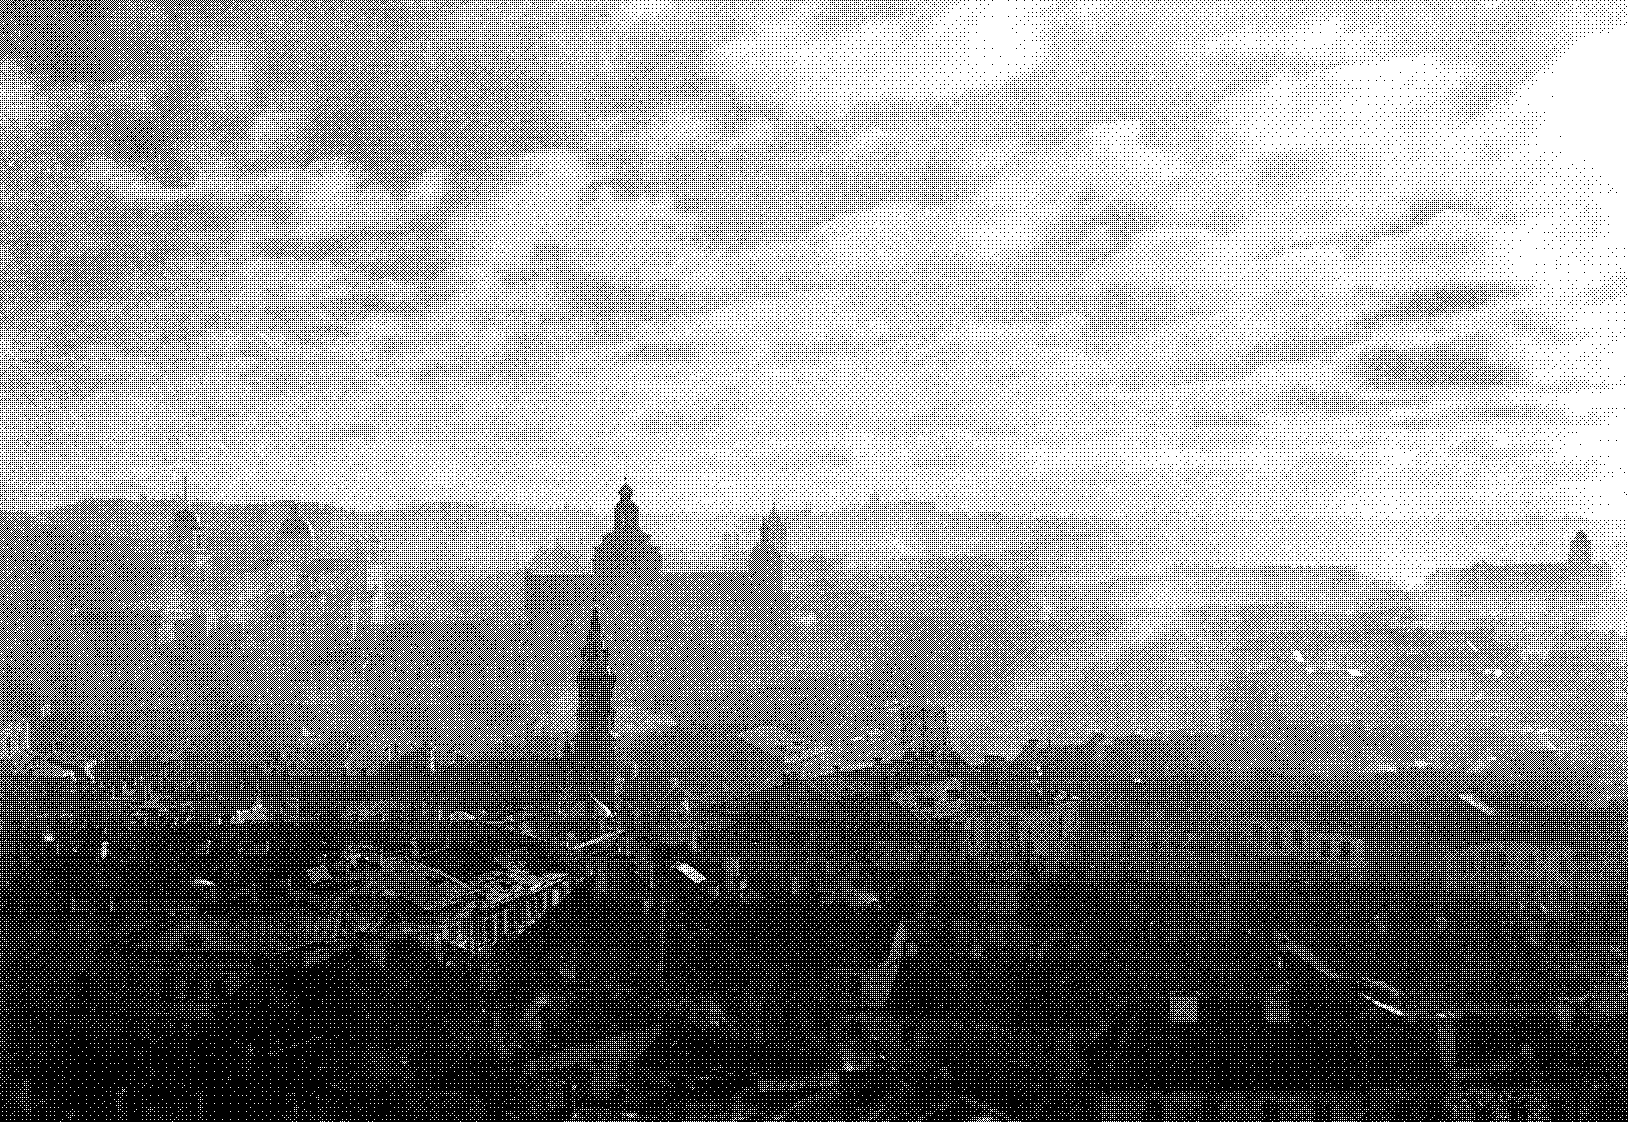
\includegraphics[width=\textwidth]{ilustra-01.png}
    \caption{Cidade velha de Vilna, por volta de 1939.}
\end{figure}

Os diversos grupos étnicos que assinalaram, no correr dos tempos, a
composição demográfica da cidade, articularam, em suas respectivas
línguas, sua compreensão histórica do que é hoje \textit{Vilnius}. Foi o que
induziu Laimonas Briedis a escrever \textit{Poetic Cartography:
 Bobrowski, Miłosz, Sutzkever}, publicado em 2015.\footnote{Laimonas Briedis.
  \textit{Poetic Cartography: Bobrowski, Miłosz, Sutzkever}. \textit{Vilnius}: \textit{Vilnius} University, 2015.} Nele examina
o papel da cidade como fonte inspiradora da criação poética de Bobrowski, escritor de língua alemã que não viveu em \textit{Vilnius}, mas a cidade é
parte do simbolismo que a ela atribuiu na História e na Geografia da
Europa Oriental. De Miłosz --- que já mencionei ---, poeta da língua
polonesa, que experienciou o exílio, iniciado quando jovem deixou a
Lituânia. E de Sutzkever, poeta da língua iídiche, que viveu no gueto de
Vilna a presença nazista na cidade. As biografias e a poesia dos três
são muito distintas, mas a cidade integra suas destilações poéticas. Na
avaliação de Laimonas Briedis, para Miłosz, \textit{Vilnius} é um local de
memória da normalidade de vida; para Bobrowski, o local das não
realizadas possibilidades da normalidade de vida; para Sutzkever, o
local das anormalidades de vida.\footnote{\textit{Idem, ibid.}, p. 89.}


Em todos os três, a experiência de base da perda e da dor provém do fato
de que as rupturas do século \textsc{xx} fizeram, como analisou Hannah Arendt,
com que a política determinasse, independentemente de suas vontades, os
rumos de vida, como, aliás, para tantas pessoas na Europa e da Europa.
Os três foram, assim, para Laimonas Briedis, uma chave para a
compreensão da complexidade de uma cidade que ele não vivenciou e que
não tem uma identidade de fácil ou inequívoca definição.

Hannah Arendt destacou em sua obra, a partir de sua experiência
reflexiva a respeito das rupturas inerentes aos extremos do século \textsc{xx}, o
poder redentor e esclarecedor da narrativa.

Numa época de ``universais fugidios'', a narrativa, em conjunto com a
pluralidade e a natalidade, configura as facetas constitutivas da ação
humana. No curso que com ela fiz, em 1965, na Universidade de Cornell, e
em outros escritos, Arendt deu ênfase ao que Kant denominou a
``mentalidade alargada'', que permite pensar no lugar de outros. Isso
requer um tipo de imaginação que enseja levar em conta a perspectiva dos
outros e de suas circunstâncias. É um \textit{go visiting} --- um ``sair em
visita'' --- que torna presente o ponto de vista dos que estão
ausentes.\footnote{Celso Lafer, ``Experiência, ação e narrativa:
  reflexão sobre um curso de Hannah Arendt''. Em \textit{Hannah Arendt:
  pensamento, persuasão e poder}. Rio de Janeiro:
  Paz e Terra, 2018, pp. 51--73.}

Faço esta remissão a Hannah Arendt porque ela contribui para destacar o
mérito e a amplitude com a qual Laimonas Briedis ``saiu em visita'' para
elaborar o juízo reflexivo de sua narrativa do percurso no tempo da
cidade de \textit{Vilnius} e da multiplicidade de perspectivas dos que nela
viveram.

George Steiner, ao escrever sobre \textit{A ideia de Europa}\footnote{George Steiner, 
\textit{A ideia de Europa}. Lisboa: Relógio d'Água, 
2017, pp. 30--32.}, aponta que
são elementos do pensamento e da sensibilidade europeia a ordem e a
cadência de seus caminhantes em seus diversificados itinerários no
espaço de sua região.

São os itinerários dos caminhantes que passaram ou viveram em \textit{Vilnius}
que nortearam, com sensibilidade europeia, o ``sair em visita'' de
Laimonas Briedis na construção de sua narrativa.

A narrativa de Laimonas Briedis é um tecido de qualidade literária que
entrelaça com originalidade a trama e o urdume. O ``urdume'' explica as
grandes forças políticas e movimentos demográficos que situaram a
Lituânia, desde suas origens, no limiar da Europa e suas vicissitudes. O
autor desvenda"-as pelo sagaz uso da cartografia e de suas dimensões
históricas com um acurado conhecimento da geografia humana. É muito
instigante o uso que sabe fazer dos mapas. A ``trama'' revela os nexos de
sentido da compreensão transversal dos fios da vida inserida no correr
dos séculos no urdume. O autor ilumina esses nexos de sentido pelos
relatos de pessoas de distintas procedências que viveram ou passaram
pela cidade e que escreveram em mais de uma língua sobre suas
experiências na cidade, a partir de suas sensibilidades e perspectivas.
A escolha desses relatos é fruto de uma garimpagem literária e cultural
de sensibilidade e abertura que deslinda o alcance geral da
particularidade de Vilna. Daí a \textit{vis atractiva} desta obra que se
insere no patamar de qualidade do gênero literário de livros sobre
cidades. Em síntese, Laimonas Briedis soube nomear e honrar, para evocar
novamente o poema de Miłosz, ``A city without a name/\,if so many are
dead''.

\section*{O legado dos \textit{litvaks}}

Quero acrescentar a este prefácio uma nota pessoal, explicitando a
origem de meu interesse por \textit{Vilna, cidade dos outros}. Conheci
pessoalmente Laimonas Briedis e tomei conhecimento de seu livro em sua
palestra ``\textit{Vilnius} e o mundo'', proferida em maio de 2018, na primeira
edição do Labas, o festival da Lituânia, em São Paulo.

O Labas ocorreu na Casa Museu Ema Klabin, da qual sou
presidente. Foi fruto de uma parceria com o Consulado Geral da Lituânia.
Resultou de uma iniciativa da Cônsul"-geral Laura Tupe, que, com suas
qualificadas atividades, colocou a presença da Lituânia no mapa de São
Paulo, inclusive em sua dimensão cultural. O Labas também respondeu a um
meritório propósito da Lituânia independente e autônoma: o de resguardar
e preservar a memória da \textit{Vilnè} judaica, que desapareceu com o
Holocausto, mas foi durante séculos um centro irradiador do conhecimento
e dos valores judaicos.

Desta \textit{Vilnè} trata Laimonas Briedis no tecido de sua narrativa sobre a
cidade. Por isso, sua palestra deu o alcance mais abrangente da mostra
fotográfica \textit{Momentos da História dos judeus na Lituânia}, que
ocorreu durante o Festival Labas, realizado na Casa Museu Ema Klabin.

A família Klabin"-Lafer, como já mencionado, é originária da comunidade
judaica da Lituânia. Imigrou para o Brasil na última década do século
\textsc{xix} e em nosso país encontrou seu destino e seus diversificados caminhos
em todas as esferas da vida nacional. Hessel Klabin, pai de Ema Klabin,
que criou a Fundação, nasceu em Zelva, na Lituânia, assim como seu irmão
Mauricio, o patrono inaugural da família no Brasil. Mauricio e Hessel
foram fundadores, em 1899, da empresa Klabin Irmãos e Cia. Leão Klabin,
pai de Hessel e de Mauricio, assim como o tio Selman Lafer, meu bisavô,
também nasceu lá e se radicou no Brasil. Nos registros familiares, a
primeira geração identificada remonta a Eliezer Lafer, também conhecido
como Eliezer Klabin, que nasceu em Zelva, em 1780. Eram assim
\textit{litvaks}, termo que designa, como já apontado, os judeus
\textit{ashkenazim} que viveram durante séculos em \textit{Litè} --- a Lituânia em
iídiche ---, uma região que é mais abrangente que o atual território da
Lituânia, pelas razões que Laimonas Briedis esclarece em sua narrativa.

No âmbito do léxico da família, enraizada no Brasil desde o início da
República, a memória da vida na Lituânia era muito tênue.\footnote{Roney Cytrynowicz. 
\textit{Mauricio Klabin: empreendedor e pioneiro da indústria brasileira}. São Paulo: Narrativa 
Um, 2019, Capítulo 1.} Teve, no entanto, presença no testamento de
Hessel Klabin, pai de Ema, escrito em São Paulo e datado de 10 de março
de 1937. Nesse testamento, que consta dos arquivos da Fundação, Hessel
instituiu pequenos legados aos israelitas pobres de Zelva, ao templo de
Bet Hamadras, a Aron Meinek e Chaim Meinek, todos de Zelva. O documento
foi subsequentemente revogado, pois as pessoas e as realidades que ele
contemplou em 1937 deixaram de existir depois do Holocausto. Hessel
elaborou seu novo testamento à luz de outras circunstâncias e faleceu em
São Paulo, em 1946.

Meus interesses intelectuais de professor universitário e homem público
são múltiplos e diversificados. No entanto, neles teve espaço a
curiosidade pelo mundo judaico da Lituânia, que está na origem de minha
família. Essa curiosidade foi alimentada pela importância da ação dos
\textit{litvaks}, que fizeram de \textit{Vilnè}, a Jerusalém da Lituânia, como já
mencionei, um centro irradiador das múltiplas dimensões do judaísmo.

Essa irradiação transita pela qualidade da exegese rabínica, da qual o
Gaon de Vilna foi notável expoente, e pelo vigor da religiosidade dos
\textit{hassidims}. Tem, entre seus componentes significativos, a
codificação do cânone literário do iídiche --- a língua materna de meus
ancestrais ---, que foi a base da criatividade artística da rica
literatura iídiche --- reconhecida pelo prêmio Nobel concedido a Bashevis
Singer.\footnote{Jacó Guinsburg, \textit{Aventuras de uma língua
  errante}. São Paulo: Perspectiva, 1996.} Em \textit{Vilnè} e em sua
efervescência, originaram"-se os movimentos sociais seculares do judaísmo
que tiveram papel nas dinâmicas do sionismo e do socialismo no século
\textsc{xx}.

Daí meu interesse pela palestra de Laimonas Briedis e a subsequente
atenção com a qual li seu livro, que insere \textit{Vilnè} na moldura mais ampla
do percurso histórico da cidade e da Lituânia. Devo registrar que o pano
de fundo que me permitiu apreciar a empreitada de Laimonas Briedis se
viu favorecido pela leitura anterior do livro de Henri Minczeles,
\textit{Vilna, Wilno, \textit{Vilnius}, La Jérusalem de Lituanie},\footnote{Henri
  Minczeles. \textit{Vilna, Wilno, \textit{Vilnius}, La Jérusalem de Lituanie}. Paris: La Découverte, 2000.} e da obra que este escreveu em
parceria com Yves Plasseraud e Suzanne Pourchier, \textit{Les Litvaks: 
L'héritage universel d'un monde juif disparu}.\footnote{Henri Minczeles;
  Yves Plasseraud; Suzanne Pourchier. \textit{Les Litvaks: L'héritage universel d'un monde juif disparu}. Paris: La Découverte, 2008.}

A este pano de fundo de leituras e conhecimentos sobre o legado
proveniente da herança dos \textit{litvaks}, sobre os quais Minczeles e
muitos outros escreveram, cabe acrescentar que estive em \textit{Vilnius} em
duas ocasiões e conheci a bonita cidade tão distante do Brasil, sobre a
qual Laimonas Briedis escreveu.

A primeira viagem foi em novembro de 2002, quando fiz, como Ministro das
Relações Exteriores, uma visita de trabalho à Lituânia, cuja
independência o Brasil tinha reconhecido em 1991 e com ela estabelecido
relações diplomáticas. Uma de minhas motivações como Chanceler e
estudioso das relações internacionais foi avaliar, na dinâmica do
funcionamento do sistema internacional, o impacto do fim da Guerra Fria
e da desagregação da União Soviética --- um tema importante para a
condução da política externa. No caso da Lituânia, como também já
mencionei, isso se traduziu no término político e econômico do Leste
Europeu e do prévio papel do país como parte integrante do bloco
soviético. Isso ensejou à Lituânia, para recorrer a um conceito de Helio
Jaguaribe, as condições de permissibilidade para atuar com viabilidade,
à luz dos próprios interesses, na condução de sua política interna e
externa.

Este foi um fato novo na vida do país, à luz do percurso de que trata
Laimonas Briedis em sua narrativa, e é um dado da dinâmica do contexto
político e diplomático da vizinhança que inseriu a Lituânia no limiar
das marchas e contramarchas da Europa Oriental.

Subjacente aos interesses diplomáticos dessa ida a \textit{Vilnius} em 2002,
estava a sensibilidade de ver a cidade na qual se deu a destruição, com
o Holocausto, da Jerusalém da Lituânia. O poeta da língua iídiche e
resistente Sutzkever vivenciou"-a no gueto de Vilna e testemunhou, em sua
criação poética, a desintegração desse mundo, como analisa com
sensibilidade Laimonas Briedis em seu já mencionado livro \textit{Poetic
Cartography}.

Foi o que me levou a fazer, oficialmente, uma visita à floresta de
Ponar, que foi o cenário da execução em massa de dezenas de milhares de
judeus. ``No Mercy in the cloud above Ponar'' é como ela aparece no
poema ``Farewell'', de Sutzkever.\footnote{\textit{Apud} Laimonas Briedis.
  \textit{Poetic Cartography}, \textit{op. cit.}, p. 175. A citação que aparece no poema ``Farewell'', ou ``Adeus'', pode ser traduzida como ``Sem misericórdia na nuvem acima de Ponar''.} No poema de
Miłosz, ``A city without a name'', que já evoquei, a passagem que cabe
lembrar é: ``What shepherd's horn swathed in the bark of birch/\,Will
sound in the Ponary Hills the memory of the absent?''.\footnote{Czeslaw
  Miłosz. \textit{Selected and Last Poems --- 1931--2004}, \textit{op.
  cit.}, p. 261. A tradução pode ser apresentada como ``O chifre de pastor envolvido na casca da bétula/\,Soará nas Colinas de Ponar a memória dos ausentes?''}

Também fiz uma visita particular a Zelva, o \textit{shtetl} originário da
família Klabin"-Lafer. É uma pequena cidade que provavelmente se
assemelha, em sua disposição urbana, àquela da qual partiram meus
antepassados. Na escola da cidade, há um pequeno museu sobre os
\textit{litvaks} de Zelva, cuja existência se deve à iniciativa de Zita
Kriaučiūnienė, professora da escola e atualmente sua diretora, que foi
grata ao apoio que em sua vida recebeu da comunidade judaica. A
instituição à qual se dedicam a professora Zita e a professora Rasa
Povylienė registra os \textit{litvaks} da cidade que se dispersaram pelo
mundo. Entre eles, os Klabin"-Lafer. O museu recolhe as informações
transmitidas por Fernando Klabin, o tradutor deste livro, que foi o
primeiro da família a visitar Zelva, na década de 1990.

Minha segunda viagem foi em novembro de 2019. Teve como objetivo
participar da inauguração da exposição ``Um modernista brasileiro de
\textit{Vilnius}: o retorno de Lasar Segall''. A exposição foi uma iniciativa do
Museu Estatal Judaico Gaon de Vilna e de sua diretora Kamilè Rupeikaitè.
Contou com o apoio da Cônsul"-geral em São Paulo, Laura Tupe. Foi um
desdobramento da primeira edição do Festival Labas e integrou os
propósitos da recuperação da memória judaica na Lituânia. Resultou de
uma frutífera parceria com o Museu Lasar Segall de São Paulo, conduzida
por seu diretor, na época, Giancarlo Hannud.

O Museu Lasar Segall, cujo Conselho integro, é hoje um museu federal
brasileiro. Teve, no entanto, suas origens nas iniciativas de Jenny
Klabin Segall, a viúva de Lasar Segall, a filha de Mauricio Klabin. Daí
a proximidade da família com as atividades do Museu.

Lasar Segall nasceu em Vilna, em 1889. É um dos grandes artistas
plásticos do século \textsc{xx}. Era um \textit{litvak}, que iniciou sua formação
artística em sua cidade natal e a ela deu densidade e continuidade na
Alemanha a partir de 1906. Participou ativamente do expressionismo
alemão, do qual foi um de seus principais expoentes. Radicou"-se no
Brasil em 1923, constituindo família ao casar"-se com Jenny Klabin.
Tornou"-se, até seu falecimento em 1957, uma irradiadora figura de proa
do modernismo brasileiro. Daí a primeira parte do título da exposição,
``Um modernista brasileiro de \textit{Vilnius}''.

A segunda parte do título da exposição, ``o retorno de Lasar Segall'',
assinala a presença de sua obra na cidade na qual esteve pela última vez
em 1918, visitando sua família, que depois veio para o Brasil. Dessa
visita, resultou o álbum de 1919, \textit{Recordações de Vilna}.

A obra de Segall, como expus em um livro dedicado a suas realizações
artísticas,\footnote{Celso Lafer. \textit{Lasar Segall: múltiplos
  olhares}. São Paulo: Imprensa Oficial, 2015.} traduz a criatividade
hermenêutica de seus múltiplos olhares. Entre eles, seu olhar sobre a
\textit{Vilnius} em que viveu. De sua cidade natal, guardou memória, registrando
em suas recordações que as impressões da cidade se refletiram em sua
obra. Daí o significado de seu retorno sob os auspícios do Museu Estatal
Judaico Gaon de Vilna, pois seu olhar sobre a \textit{Vilnè} judaica é parte dos
fios do tecido da narrativa do livro de Laimonas Briedis.

Segall integra o rol dos muitos artistas plásticos que se dispersaram
pelo mundo com a diáspora dos \textit{litvaks} no século \textsc{xx}. A preservação
da memória de suas realizações artísticas é parte dos propósitos do
governo da Lituânia de manter vivo o que foi o alcance de sua herança
judaica. Foi nesse contexto que, nessa minha ida à Lituânia em 2019,
recebi um importante e ilustrado livro, publicado em \textit{Vilnius} em 2015,
\textit{Litvak Art}, que elenca esses artistas --- inclusive Segall --- e
reproduz muitas de suas obras.

Nessa viagem, junto com os netos de Lasar Segall e outros membros da
família, tive a oportunidade de ver muitos dos remanescentes locais de
memória da Jerusalém da Lituânia, o que propiciou uma visão concreta de
facetas da narrativa do livro de Laimonas Briedis.

A viagem de 2019 foi uma viagem de família. Foi o que nos levou, além de
apreciar \textit{Vilnius} e a exposição de Segall, a também fazer uma visita a
Zelva, o local de origem da família, onde estive em minha ida em 2002.
Nesse sentido, constituiu"-se como um resgate da memória muito distante e
esmaecida da origem \textit{litvak} da família, que foi um desdobramento
do Labas de 2018, no qual conheci o autor do livro.

\section{De Mickiewicz a Machado de Assis}

Uma palavra final. Para a edição brasileira, Laimonas Briedis escreveu
a introdução ``Vilna no Brasil''. É um relato de sua experiência de
viagem ao nosso país por ocasião do Festival Labas de 2018. Nela examina
com sensibilidade os contrastes entre dois países distintos, mas também
explora proximidades, por exemplo, as provenientes do vocabulário do
barroco. Compreensivelmente, a reflexão sobre a obra de Segall é uma de
suas trilhas de entendimento, em especial quando descreve a beleza da
natureza de seu país e identifica nas florestas de Segall a filtragem
das cores da Lituânia.

O prefácio tem epígrafes, as quais usualmente estendem e apontam a
atmosfera que permeia um texto. A primeira é de Machado de Assis,
extraída de \textit{Dom Casmurro}: ``Mas a saudade é isto mesmo: é o
passar e o repassar das memórias antigas''.

O livro de Laimonas Briedis é uma narrativa que passa e repassa com
originalidade a memória das vicissitudes do percurso histórico de sua
cidade natal.

A epígrafe de Machado de Assis remete para o tema da saudade, uma
palavra que é uma peculiaridade da língua portuguesa, para a qual
Laimonas Briedis procura correspondências em lituano e também para as
subjacentes saudades que se originaram do percurso histórico de \textit{Vilnius}.

El Rei D. Duarte, em \textit{Leal Conselheiro}, livro escrito no século \textsc{xv}, 
foi o primeiro a tratar da saudade em nossa língua. Em sua análise, por assim dizer
fenomenológica, de sua problemática, diz que a saudade é um sentimento
que provém do coração e da sensibilidade, não da razão. Origina"-se do
apartamento de pessoas, lugares ou coisas pelos quais se tem afeição. A
saudade pode trazer o prazer da boa lembrança. Pode manifestar o
desprazer e a tristeza do mal e da impossibilidade de regresso em
relação àquilo pelo qual se teve afeição.

O poema de Sutzkever, ``Iídiche de Vilna'', que é a segunda epígrafe do
prefácio, destila a expressão poética da saudade triste e sem regresso,
do fim da Jerusalém da Lituânia que ele presenciou, cuja existência no
passado integra a narrativa de Laimonas Briedis.

Em minha viagem de 2019, recebi o \textit{Álbum"-Catálogo} de
pôsteres do gueto de Vilna. Publicado pelo Museu Estatal Judaico Gaon de
Vilna,\footnote{\textit{Album"-Cathalogue Vilna Ghetto Posters}. Vilna: Baltos Lankos, 2005.} o 
\textit{Álbum"-Catálogo}, impacta. Visualiza relances da resiliência
resistente da vida cultural judaica dos \textit{litvaks}, da qual
Sutzkever participou, nas terríveis condições do gueto.

Em sua introdução, Laimonas Briedis evoca Machado de Assis, nossa
maior referência literária, para trazer com sagacidade a Lituânia para
o Brasil. Machado teve interesse pelo poeta polonês Adam Mickiewicz, que
nasceu na região da Lituânia, hoje situada na Bielorrússia. Estudou na
Universidade de Vilna, que foi, em sua época, na \textit{heteroglossia} da
cidade, um espaço de criatividade literária da língua polonesa. Por suas
atividades em sociedades estudantis polonesas patrióticas, foi banido
pelas autoridades russas czaristas. Tornou"-se um arauto defensor da
perdida independência da Polônia e viveu exilado em Paris.

Machado, a partir do francês, traduziu seu poema ``Alpujarra'', que
figura na primeira edição de \textit{Crisálidas}. O poema trata dos
embates entre mouros e castelhanos na Península Ibérica. Na introdução,
explica Laimonas Briedis que se trata de uma balada inserida num poema
mais longo, de enredo complexo, que descreve as lutas dos lituanos
pagãos contra os cruzados na Idade Média. Remete, assim, para sua
sensibilidade, como um contraponto, à inserção da Lituânia em seu limiar
na Europa, que integra a narrativa de seu livro.

Machado, em suas crônicas, teve interesse pelos fatos políticos
nacionais e internacionais. Em \textit{Crisálidas}, figura o poema
``Polônia'', que tem como epígrafe uma citação de Mickiewicz e antevê a
ressurreição da independência da Polônia, que dela foi privada nas
marchas e contramarchas da política europeia do século \textsc{xix}.

Laimonas Briedis destaca que a poesia de Mickiewicz, na descrição da
natureza que configurou grande parte de sua obra criada no exílio, se
inspira na paisagem nativa de sua Lituânia natal. Inclusive o celebrado
rio que aparece no poema ``Polônia'' de Machado de Assis é o Niemen da
Lituânia, do qual é tributário o rio Neris, que fica nas margens de
\textit{Vilnius}, também conhecido em iídiche (como em polonês) como o rio
Viliya, e é assim que aparece no poema de Sutzkever evocado na epígrafe.
Em síntese, o tema do rio e da natureza que aparece na poesia de
Mickiewicz, que tocou Machado de Assis, é também o da saudade das
paragens da Lituânia. É assim, sob os auspícios de Machado de Assis, que
Laimonas Briedis encerra seu prefácio, inserindo a Vilna de seu livro no
Brasil, tornando mais uma vez próximo o distante.

%São Paulo, novembro de 2020.
